\documentclass[10pt]{article}
\usepackage[T1]{fontenc}\usepackage{lmodern,amsmath,amssymb,graphicx,hyperref}
\usepackage[margin=.75in]{geometry}
\setlength{\parindent}{0pt}\setlength{\parskip}{7pt}
\begin{document}
\begin{center}{\Large Common-profile content at arbitrary retained charts}\\[4pt]
Local continuation --- 15 November 2026\end{center}
\textbf{Result.} Use one common multiplicity profile $m_j=4n_j$, with
arbitrary natural $n$. Let $t$ be an actual nonzero retained integer node
in the grid, with actual valuation $i=v_2(t)<u\le a$. For every residue,
every column and every admissible odd moment $2b+1<k$, the full actual
right polynomial satisfies
\[
 \operatorname{Content}_{q_i} R_{t,(r,2b+1),y}(Z),\qquad
 q_i=\min\{2,u-i-1\}.
\]
This covers positive-anchor zeros as well as negative nodes, without a
favorable local numerator or jet-unit premise [pcc:unverified].

\begin{center}\begin{tabular}{c|c}
Retained valuation level & Guaranteed extra right content\\\hline
$i\le u-3$ & two bits\\
$i=u-2$ & one bit\\
$i=u-1$ & zero bits
\end{tabular}\end{center}

\textbf{Actual integral instance.} Work in
$\mathcal A=\{x\in\mathbb Q:v_2(x)\ge0\}\cup\{0\}$, the existing
\texttt{integralRationals} subring, and coefficient ring $\mathcal A[Z]$.
Replace the moment variable $H$ by $H/2$. Actual node-half slopes have
content at least $u-i-1$; actual anchor-half slopes are integral.
The actual numerator and chart base have integral lifts. Their subtype
maps equal the \emph{same} original normalized formulas
[pcc:unverified].

\textbf{Generic law applied as stated.} For a commutative ring $R$, if
$d\mid4$ and $d\mid B$, the odd coefficients of
\[
 C(N)\sum_{v<k}(1-D)^v,\qquad
 D=(C(A)+C(B)H)\prod_{j\in S}(1+C(s_j)H)^{4n_j}
\]
are divisible by $d$. In the quotient by $(d)$, the node-linear term
vanishes and each fourth power is an even expansion. Existing polynomial
homomorphism laws preserve that expansion through the finite product and
geometric sum; the existing ideal-quotient theorem returns a divisor
witness inside $R$ [pcc:unverified].

\textbf{Transfer to the actual right factor.} Instantiate
$R=\mathcal A[Z]$, $d=2^q$ with $q\le2$ and $q\le u-i-1$.
Both divisor contracts are derived from the actual data. Mapping the
integral witness back to $\mathbb Q[Z]$ and applying existing content
multiplication gives the coefficientwise bound. The exact $H/2$
coefficient identity supplies the original $2^{-b}$ normalization.
The noncrossing branch is explicitly zero. Divisibility in
$\mathbb Q$ alone is never used as valuation evidence [pcc:unverified].

\textbf{Retained-node scope.} The node is a subtype of the existing grid
predicate, with nonzero value and explicit valuation equality. No division
by its actual numerator first jet occurs. One exact negative approximation
specialization preserves the older construction. The highest-node exception
agrees with the earlier two-node first-coefficient difference of one
[pcc:unverified].
\newpage
\begin{center}{\Large Validation and the cost connection}\end{center}
\begin{center}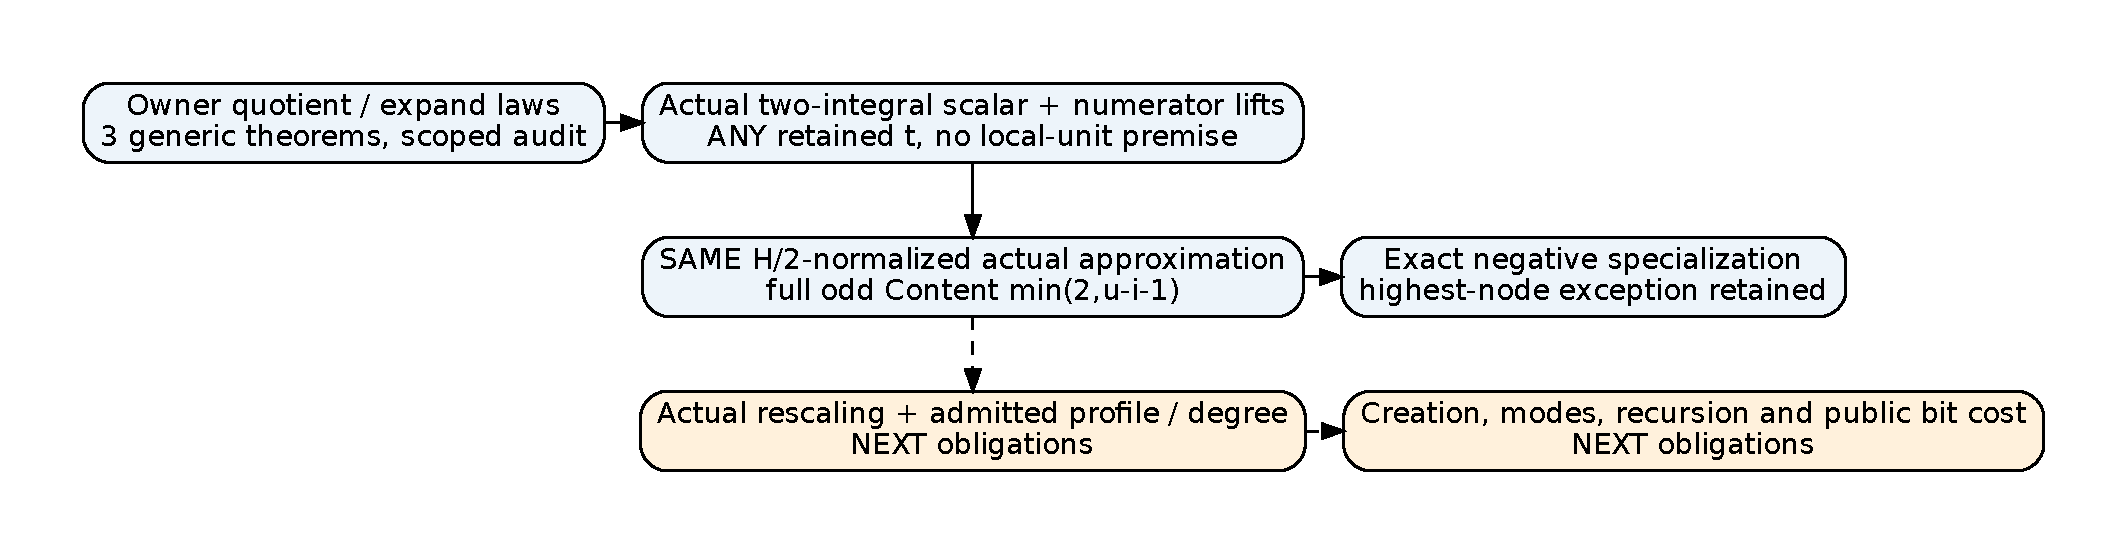
\includegraphics[width=\linewidth,height=2.25in,keepaspectratio]{retained-nonuniform-dependencies-001.pdf}\end{center}
\textbf{Accepted study evidence.} Sources102,104,105 and107 compile
441,445,447 and458 named source statements including historical parents,
all exit zero without warnings or sorryAx. Receipts054--057 bind each exact
source, raw output and exit. The19 source declarations beyond439 include
eight retained-domain generalizations and three semantic compatibility
facts, rather than19 arithmetic novelty claims. Printed central dependencies
are standard [pcc:unverified].

\textbf{Owning-library evidence.} CryptoLean commit810ae77 has three generic
quartic, quotient and finite-geometric divisor laws, including its two
previously accepted primitives. The scoped pinned module axiom auditor
reports three theorems, zero failing and zero trusted. Receipts052 and053
preserve primitive and complete-module versions. Consumer dependency pins
are unchanged; the experimental import overlay is explicit. All new claims
are unsigned and defaultnot\_covered; these local files are outside shared
Transport53/57/fresh coverage [pcc:unverified].

\textbf{Failed attempts.} Owner parity001 had a conditional-lemma name
collision. Study103 missed an owning namespace and predicate normalization;
106 required named constructor projection and valuation contracts for the
negative compatibility bridge. Every failed source, pre-call hash, compiler
output and exit is retained. The bridge was repaired rather than omitted.
No old frozen source, claim or evidence bytes were altered
[pcc:unverified].

\textbf{Next actual construction.} Apply existing matrix diagonal/unit laws
to rescale odd left factors by $2^{q_i}$ and right factors by $2^{-q_i}$
in rational polynomials before finite reduction. Derive the same product,
residual and integral factors. Then construct an actual admitted profile
and charge its exact multiplicity, mass and degree. No positive feasible
profile is constructed in this result [pcc:unverified].

\textbf{Creation and public cost.} Right division needs adequate working
precision before freezing the creation value; an old finite-ring word
cannot simply be divided by two. Charge every label, coefficient and scalar
preparation, immutable representation, child edge, retry and bit operation.
Original elliptic relation, public finder and scalar extraction remain
separate interfaces. The auxiliary $W$ and origin are unchanged; no jet
completion $H$ or nonscalar origin is constructed. A local content gain
alone gives no complete expected-cost exponent [pcc:unverified].

\textbf{Preservation.} Versioned additions only. The protected remote PCC
history still withholds publication; independent local mathematics remains
available. No native, timing, scaling, paid/cloud or attack campaign was run.
\end{document}
